In this section, we briefly introduce the issue tracking system on GitHub and the open source bounty platform Bountysource.


\subsection{Issue tracking system on GitHub}

%\begin{figure*}[t]
%   \centering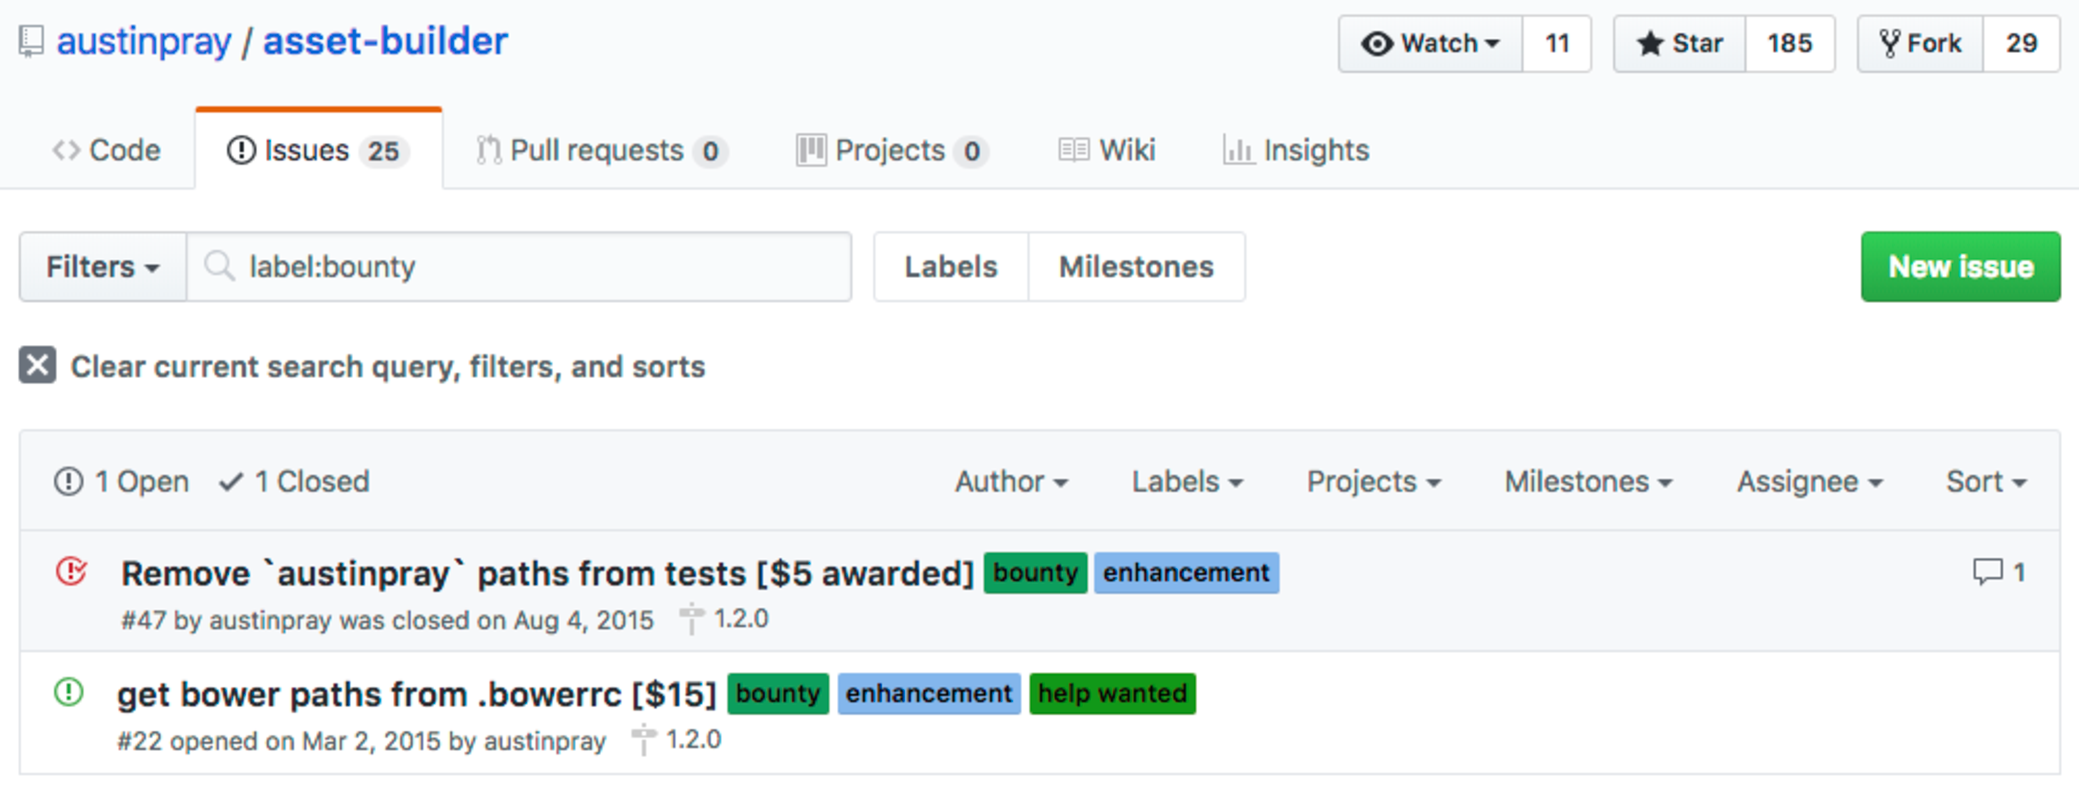
\includegraphics[width=17cm]{pics/bg/github_its}
%  \caption{Issue reports with a `bounty' label in the issue tracking system of the \code{austinpray/asset-builder} project on GitHub.}
%  \label{istdemo}
%\end{figure*}

The issue tracking system (i.e., ITS) on GitHub helps developers to manage the issue reports of their project. Users and developers can report bugs or request new features by posting an issue report on the issue tracking system. There are two statuses of an issue report: ``open'' and ``closed''. ``Open'' indicates that the issue report is still active and is waiting to be addressed. ``Closed'' indicates that the issue report has been closed. The most common reason for closing an issue report is that the issue has been addressed, but it could also have other reasons (e.g., duplicated issue reports).
Users can attach free-text labels to issue reports to indicate the category of an issue report.
An issue report contains a title to summarize the issue and a description that describes the issue in detail.
Developers can discuss an issue report by leaving comments, which can include code snippets, links or images to improve the description.
%For example, Figure~\ref{istdemo} lists two bounty issues\footnote{\url{https://github.com/austinpray/asset-builder/issues?q=label\%3Abounty}} of the \code{austinpray/asset-builder} project on GitHub. Both issues are tagged with the ``bounty'' label.



\subsection{Bountysource}
Bountysource is a platform on which users can pledge a monetary incentive (a \textit{bounty}) to address an issue report of an open source project.
There exist two roles on Bountysource: the bounty backer and the bounty hunter roles.

\noindent\textbf{Bounty backers}, which may be anonymous, are users or developers who propose bounties for issue reports. The backer can set an expiration period for bounties that are over \$100. When the bounty expires, the money is refunded to the backer; otherwise, the bounty stays with the issue report until someone claims it. Bounties that are smaller than \$100 are not refunded if they remain unclaimed. An issue report can have multiple bounties from one or more backers.

\noindent\textbf{Bounty hunters} are developers who address issue reports that have bounties. Once a developer claims to have addressed an issue report, its bounty backer(s) can choose to accept (no response will be taken as an acceptance) or reject the claim. In this situation, backers have two weeks to make the decision (accept or reject). If no backer explicitly rejects the claim, the bounties will be paid to the developer automatically.
Multiple bounty hunters can work on an issue report at the same time, but the bounties of an issue can only be rewarded to one bounty hunter.






Figure~\ref{RelationEntity} summarizes the relationships between the bounty, the bounty backer, the bounty hunter, the issue report, the issue reporter, and the developer. Basically, when an issue report is submitted by an issue reporter, one or more bounty backers can propose bounty(ies) on the issue report. One or more developers of the issue report can choose to become bounty hunters to address the issue report but only one bounty hunter can get the bounty(ies).




\begin{figure}[t]
   \centering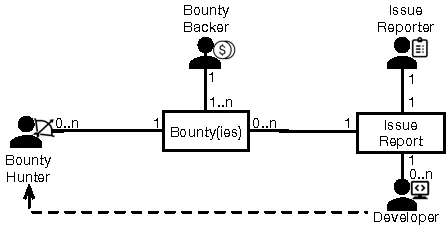
\includegraphics{pics/bg/RelationEntity}
      \vspace{-0.1in}
  \caption{The relationships between entities that are involved in the  bounty process.}
  \label{RelationEntity}
  \vspace{-0.1in}

\end{figure}

%There are two kinds of backer in Bountysource: 1) the personal backer, which represents an individual user. 2) The team backer, who represents a team or company (e.g., IBM).


Developers and users from more than 12 platforms (e.g., GitHub) propose bounties for issue reports through Bountysource. In this study, we focus on GitHub issue reports, since the majority of the bounties (see Section~\ref{dataset} for more details) that are proposed on Bountysource are for GitHub issue reports.
Figure~\ref{bountyflow} shows the workflow of the bounty processes between GitHub and Bountysource.
The lifecycle of a bounty starts with a bounty backer proposing a bounty for an issue report on GitHub. Bountysource will generate a link to the issue report on GitHub.
The bounty backers pledge money to Bountysource (the money is held by Bountysource) and can choose to ``advertise'' the bounty by tagging the issue report on GitHub with a bounty label (see the example\footnote{\url{%https://github.com/austinpray/asset-builder/issues?q=label\%3Abounty
http://bit.ly/2EQEA6c}} for details), appending the bounty value to the title of the issue report or mentioning the bounty in the discussion of the issue report in GitHub.
When a bounty hunter starts working on an issue, they can update their working status on Bountysource.
After the issue report is addressed, the bounty hunter can submit a claim for the bounty on Bountysource and the backer will be notified.
Once the bounty backer accepts the claim, the bounty hunter receives the money from Bountysource.

\begin{figure}[t]
   \centering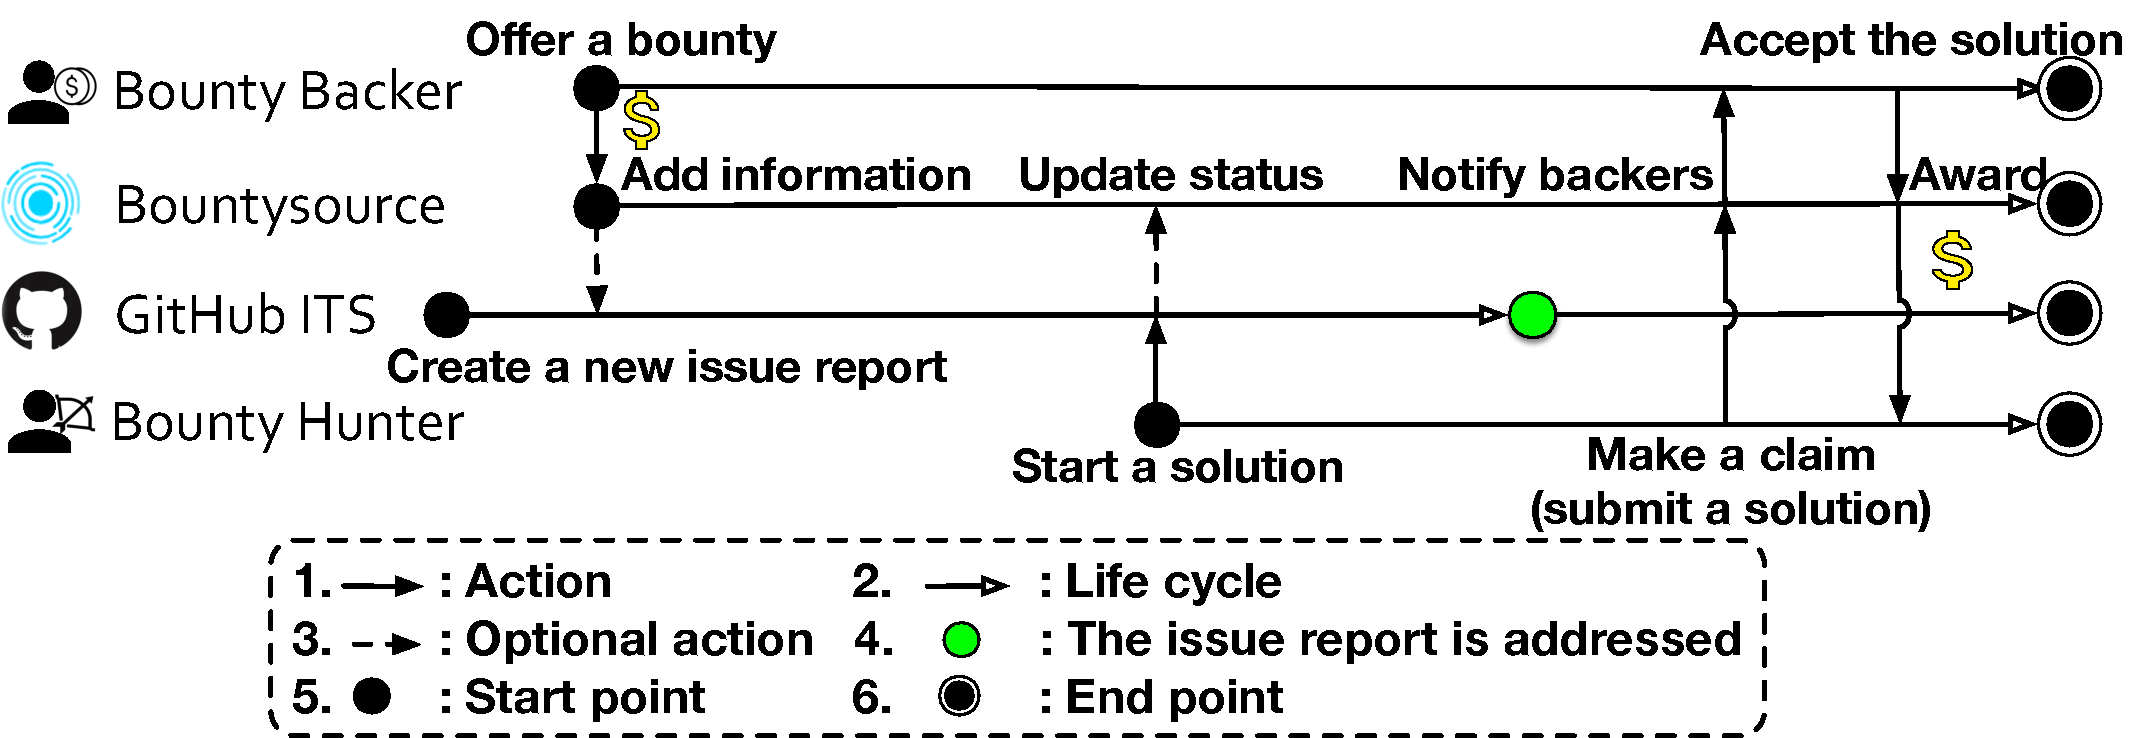
\includegraphics[width=9cm]{pics/bg/bountyflow}
   \vspace{-0.2in}
  \caption{The workflow of the bounty between GitHub and Bountysource.}
  \label{bountyflow}
  \vspace{-0.1in}

\end{figure}

Based on the status of an issue report and whether a bounty is paid out, a bounty issue report has the following three statuses:

\noindent\textbf{Closed-paid}: the issue report is closed and the bounty has been successfully rewarded to a bounty hunter. We defined such issue reports as \emph{successful} bounty issue reports.

\noindent\textbf{Open-unpaid}: the issue report is open and the bounty is active. We defined such issue reports as \emph{failed} bounty issue reports.

\noindent\textbf{Closed-unpaid}: the issue report is closed but the bounty remains unclaimed. We defined such issue reports as \emph{ignored} bounty issue reports.




